\section{Summary}

aLIGO has begun taking data and will achieve design sensitivity over the next few years. At that point, the next generation of upgrades and improvements must be nearly ready to implement. One possible such upgrade would be to damp the unwanted angular motion in the test masses using radiation pressure feedback. This has the potential benefits of reducing the angular noise of the system and thus also reducing the amount of noise that couples from angular motion into cavity length.  
 
We have explored the implementation and uses of radiation pressure feedback, optical springs, to control the motion of a mirror. 
We demonstrated in several ways the underlying principles and behavior of optical springs, in both straight and folded cavities.
We discussed the mechanical design of the experiment, with the addition of blade springs to reduce the influence of seismic noise on the experiment.
We reviewed the feedback and controls in use for the optical traps. 
We measured and modeled the causes and effects of the photothermal effect in an optical spring system.
We explored one- and two-degree-of-freedom traps, and, while we could not get the angular trap stably locked for more than two seconds, we have laid out the path to do so.
We designed and modeled a full-scale implementation of angular optical springs to damp the Sidles-Sigg instability in the aLIGO configuration.

These developments should lay a strong groundwork for continued research into the applications and uses of radiation pressure feedback in aLIGO and beyond.

\section{Future work}

There are several things left unfinished that will hopefully deliver interesting results:

\begin{enumerate}
	\item Improving the stability  of the SU angular optical trap experiment and damping the 66 Hz resonance that seems to be preventing extended locks.
	There are a number of possibilities to increase the bandwidth and damp the motion outlined in Section \ref{sec:bandwidth}.
	\item Exploring the possibility of a a single stable optical spring with a specialized optical coating.
	We expect that dielectric coating manufacturers could do a custom run with a very thick first layer to create a ``self-locking'' cavity. The mirror could be mounted using the same cold weld method described in Section \ref{sec:endMirror}, then tested with the single-mirror input coupler from Chapter \ref{ch:photothermal}. 
	\item Designing and demonstrating a large scale angular trap in aLIGO.
	A detailed noise budget needs to be drafted using a modified version of GWINC or a similar tool to insure that we would not be introducing too much thermal noise.
	After that, a prototype of the design would need to be built at e.g. the Caltech 40 m interferometer to develop control systems and test predictions.
\end{enumerate}

%For each bullet, add at lease one more sentence that discusses how you would go about these items.
%What is the first thing to be done? What hardware needs to be purchased, changed? Etc.


%% $Id$
%
%Although the upper limit that we have placed on the rate of binary black hole
%MACHO inspirals in the galaxy is lower than the upper bound of the predicted
%rates, the LIGO interferometers were not at design sensitivity when the S2
%data was taken. At present, the sensitivities of the instruments are
%significantly better than during S2, as can be seen from
%figure~\ref{f:s3strain}, and progress on reducing noise in the interferometers
%continues apace.  The increase in detector sensitivity makes a larger volume
%of the Universe accessible to searches for binary inspirals. In addition to
%this, the amount of data is also increasing as the interferometers become more
%stable.
%
%These improvements in the instruments will increase the chance of detecting
%gravitational waves from binary inspirals. If the rates of binary black hole
%MACHO coalescence are truly as high as predicted, then initial LIGO would
%stand an excellent chance of detecting an inspiral. The first detection of
%gravitational waves will be a major scientific breakthrough and will yield and
%enormous amount of scientific information, particularly if the detection came
%from a binary black hole MACHO. The length of binary black hole MACHO
%inspirals in the sensitive band of the interferometer will allow extremely
%accurate parameter estimation as well as tests of post-Newtonian theory. For
%systems with total mass greater than $\sim 0.64\,\mathrm{M}_\odot$ LIGO will
%be sensitive to the coalescence of the binary and will be able to study the
%strong gravitational field effects when two binary black holes merge. When
%this is coupled with the accurate parameter estimation available from the
%earlier part of the waveform, the inspiral of a binary black hole MACHO could
%be an excellent laboratory for General Relativity.  A detection would also
%impact the studies of halo dark matter and early universe physics, providing a
%MACHO component to the halo and suggesting that primordial black holes do
%indeed form in the universe.
%
%In the absence of detection, the improvements in detector sensitivity will
%dramatically improve the upper limits placed on the rate of binary black hole
%MACHO inspirals. Once these rates are below the predicted rates, we may begin
%to use observations from gravitational wave interferometers to constrain the
%fraction of galactic halos in the form of primordial black hole MACHOs. While
%this may not be as significant as a detection, it will still be of interest to
%the astrophysical community.
%
%\newpage 
%
%\begin{figure}[p]
%\vspace{5pt}
%\begin{center}
%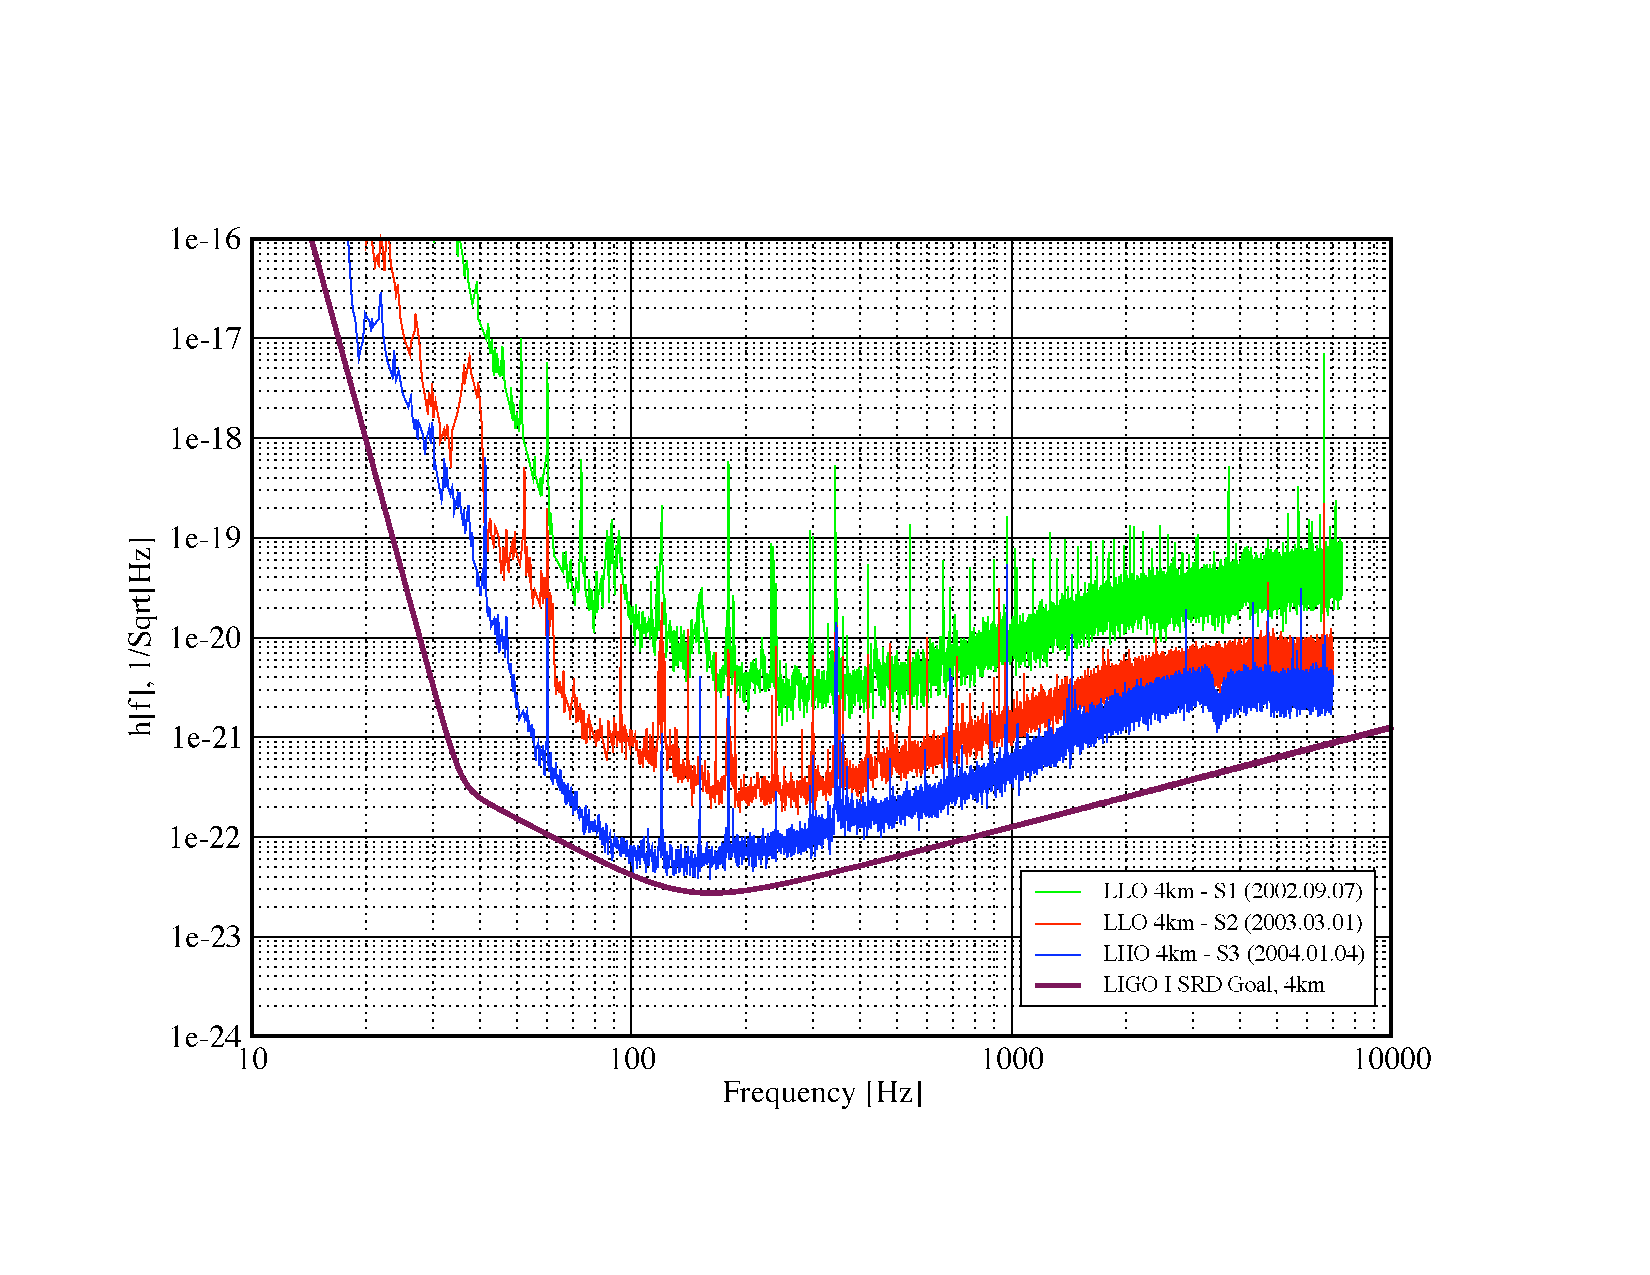
\includegraphics[width=\textwidth]{figures/conclusion/s3strain}
%\end{center}
%\caption[Comparison of Best LIGO Interferometer Sensitivity]{%
%\label{f:s3strain}
%Comparison of the best sensitivities of the LIGO interferometers between
%science runs. The solid curve shows the design sensitivity for the $4$~km
%interferometers: the LHO $4$~km is only a factor of $\sim 2$ away from design
%at $100$~Hz during S3.
%}
%\end{figure}
%
